\documentclass[12pt, titlepage]{article}
\usepackage[utf8]{inputenc}
\usepackage{booktabs}
\usepackage{tabularx}
\usepackage{graphicx}
\usepackage{hyperref}
\usepackage{enumerate}
\usepackage{soul}
\graphicspath{ {figures/} }
\usepackage{fancyhdr}
\hypersetup{
    colorlinks,
    citecolor=black,
    filecolor=black,
    linkcolor=red,
    urlcolor=blue
}
\usepackage[round]{natbib}
\usepackage{comment}

\title{SE 3XA3: Software Requirements Specification \\ Return of the Bomberman}

\author{Team \#18, REM
		\\ Miles Jackson  jacksa7
		\\ Eitan Yehuda  yehudae
		\\ Ridhwan Chowdhury chowdr11
}

\date{\today}

\begin{document}

\maketitle

\pagenumbering{roman}
\tableofcontents
\listoftables
\listoffigures

\begin{table}[bp]
\caption{\bf Revision History}
\begin{tabularx}{\textwidth}{p{3cm}p{2cm}X}
\toprule {\bf Date} & {\bf Version} & {\bf Notes}\\
\midrule
February 8, 2021 & 1.0 & First Iteration of Module Guide\\
\textcolor{red}{April 7, 2021} & \textcolor{red}{1.1} & \textcolor{red}{Added ActivePlayers Module}\\
\bottomrule
\end{tabularx}
\end{table}

\newpage

\pagenumbering{arabic}

This document describes the requirements for ROTB, which is an implementation of the Bomberman game in Javascript. The template for the Software Requirements Specification (SRS) is a subset of the Volere template. This document serves to inform users and stakeholders of the overview of the project including constraints and objectives this project hopes to meet.

\section{Project Drivers}

\subsection{The Purpose of the Project}
The purpose of ROTB is to re-implement and modify the original Bomberman game. The original implementation is incomplete, and the team will polish the base functionality of the game, while building additional features. Overall, the goal is to have a game that can be enjoyed by anyone with internet access and a computer.

\subsection{The Stakeholders}

\subsubsection{The Client}
The client for ROTB is the instructor and teaching assistants of the SFWRENG 3XA3 course.

\subsubsection{The Customers}
The customers of this project are all with an interest in the original Bomberman game and open-source game development in general. This project will be available for anyone with internet access.

\subsubsection{Other Stakeholders}
The developers and project managers have a vested interest in the completing and improving an unfinished product. This potentially includes updates and more features deployed in the development cycle.
\\ \\ \\ 

\subsection{Mandated Constraints}
\textbf{Description:} The project shall follow the structure of deliverables outlined in the project schedule. \\
\textbf{Rationale:} The project needs to follow a schedule to ensure completion of the product within the time allotted. \\
\textbf{Fit Criterion:} The project is completed and all deliverables are submitted by April 12, 2021. \\ \\
% we need to change this up haven't looked at the code yet LOL
\textbf{Description:} The project shall use Javascript as the implementation for game development. \\
\textbf{Rationale:} The project is originally written in Javascript which will make it easier to build on the implementation. \\
\textbf{Fit Criterion:} Running the game on a hosted website by any user with internet access.


\subsection{Naming Conventions and Terminology}

\begin{itemize}
    \item \textbf{OS} : Operating System
    \item \textbf{2D} : Two-Dimensional
    \item \textbf{CIA} : Confidentiality, Integrity and Availability
    \item \textbf{SFWRENG 3XA3} : The Software Engineering Practice and Experience: Software Project Management course instructed by Dr. Asghar Bokhari.
    \item \textbf{Main Menu} : The initial menu where the user can determine what they want to do in the game.
    \item \textbf{ROTB} : Return of the Bomberman
\end{itemize}

\subsection{Relevant Facts and Assumptions}
% User characteristics should go under assumptions.
Users of this product are expected to have access to a computer with a Linux based OS such as Windows or MacOS. The user is assumed to have a keyboard in order to interact with the game. Users are also expected to have a stable internet connection and access to an internet browser such as Google Chrome, Safari or Microsoft Edge.


\section{Functional Requirements}

\subsection{The Scope of the Work and the Product}


\subsubsection{The Context of the Work}

This software scope will be to build ROTB based on the original Bomberman. This project will be hosted on the internet and implemented with Javascript and HTML/CSS. Special features such as multiplayer and powerups will be implemented within this project. The goal of this project will be to replicate, build and polish ROTB from the base game of Bomberman. 

\subsubsection{Individual Product Use Cases}
\begin{figure}[h]
\centering
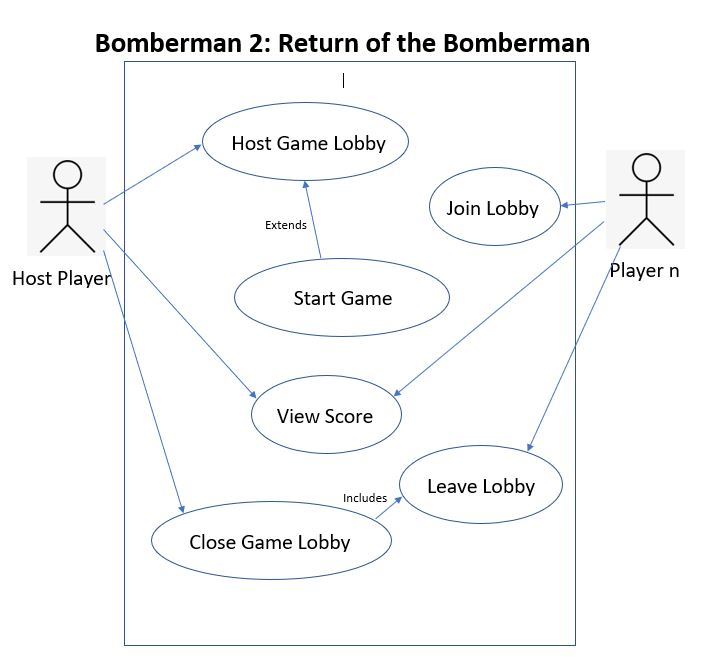
\includegraphics[width=12cm]{UseCaseDiagramServer}
\caption{Use Case Diagram}
\label{fig:figure1}
\end{figure}

A primary focus of this project is allowing a player to host a game lobby allowing up to four players to join the lobby. Once all players have joined, the host can start the game.

\subsection{Functional Requirements}
\begin{enumerate}[{FR}1. ]
    \item When the user presses the 'W' key, the character moves up one space.
    \item When the user presses the 'S' key, the character moves down one space.
    \item When the user presses the 'A' key, the character moves left one space.
    \item When the user presses the 'D' key, the character moves right one space.
    \item When the user presses the space-bar, the character drops a bomb on their current location.
    \item When the user touches a power-up, the character is able to use that respective power.
    \item A bomb shall explode after 3 seconds after being placed.
    \item The user can only place 1 bomb at a time, unless this conflicts with a power-up.
    \item Explosions shall go on the square of the bomb as well as 2 squares in each non-diagonal direction.
    \item If an explosion collides with a soft wall, the wall shall be destroyed and the explosion shall stop in the direction.
    \item If an explosion collides with a hard wall, the wall shall be remain standing and the explosion shall stop in the direction.
    \item When a player collides with a wall of any kind they shall not be able to move in that direction.
    \item When a player collides with an explosion they shall die.
    \item When only one players remains alive the game shall end, and that player shall be considered the winner.
    \item In a multiplayer game, if the host player leaves the game, \st{the game ends for all players.} \textcolor{red}{the host shall be transferred to the next person in the lobby. If no other exist the game shall end.}
    \item In a multiplayer game, \st{if any player other than the host leaves the game, that player should be treated as if they collided with a bomb.} \textcolor{red}{if any player leaves the game their character shall remain idle until a new player connects and takes their spot.}

    
\end{enumerate}

\section{Non-functional Requirements}

\subsection{Look and Feel Requirements}

\begin{enumerate}[{LR}1. ]
    \item The game must have a Bomberman theme to it and follow a consistent art style. 
    \item The game must have large text readable to most players
\end{enumerate}



\subsection{Usability and Humanity Requirements}

\begin{enumerate}[{UH}1. ]
    \item The game must use traditional 2D computer game keyboard controls such as WASD or arrow keys to move
    \item The language used in the game must be easily understandable by most English speakers.
    \item The game will be playable for people with a color vision deficiency. 
\end{enumerate}



\subsection{Performance Requirements}

\begin{enumerate}[{PR}1. ]
    \item The game must respond to control inputs within 0.2 seconds.
    \item The game must refresh at least 5 times per second.
    \item Movements by other players must be seen within 0.4 seconds.
\end{enumerate}

\subsection{Operational and Environmental Requirements}
\begin{enumerate}[{OE}1. ]
    \item The game mus run on any computer that uses Safari, Google Chrome, or Microsoft Edge as its respective browser. An internet connection will be required to play the game.
\end{enumerate}


\subsection{Maintainability and Support Requirements}

\begin{enumerate}[{MS}1. ]
    \item The game shall be maintained until May 2021, by the developers.
    \item The program must be supported by operating systems mentioned above.
\end{enumerate}

\subsection{Security Requirements}
\begin{enumerate}[{SR}1. ]
    \item The program must not have access to personal user data.
    \item The program must ensure that user data is protected by CIA Triad.
\end{enumerate}


\subsection{Cultural Requirements}
\begin{enumerate}[{CR}1. ]
    \item The game must not contain any graphic content.
    \item The game must not contain any explicit language.
\end{enumerate}

\subsection{Legal Requirements}
\begin{enumerate}[{L}1. ]
    \item This project must ensure that a valid license is provided with the original game allowing the use of original which the rest of the team improves upon.
    \item The product must not violate copyright.
\end{enumerate}

\subsection{Health and Safety Requirements}
N/A.

\section{Project Issues}

\subsection{Open Issues}

There are currently no open issues.

\subsection{Off-the-Shelf Solutions}

As this game is recreating a newer version of an existing game there are some versions of the game which can be found that are similar. Such as the official Bomberman game that was released on NES as well as the official sequels to follow. There have also been other recreate attempts that can be online such as on gameofbombs.com. Our project will use none of the code found in any of these current solutions.

\subsection{New Problems}

\subsection{Tasks}

A link to the project schedule can be found in the project repository linked below:\\

\href{https://gitlab.cas.mcmaster.ca/chowdr11/3xa3/-/tree/master/BlankProjectTemplate/ProjectSchedule}
{\textbf{Gantt Chart}}\\

\noindent This chart will be updated throughout the project

\begin{figure}[h]
\centering
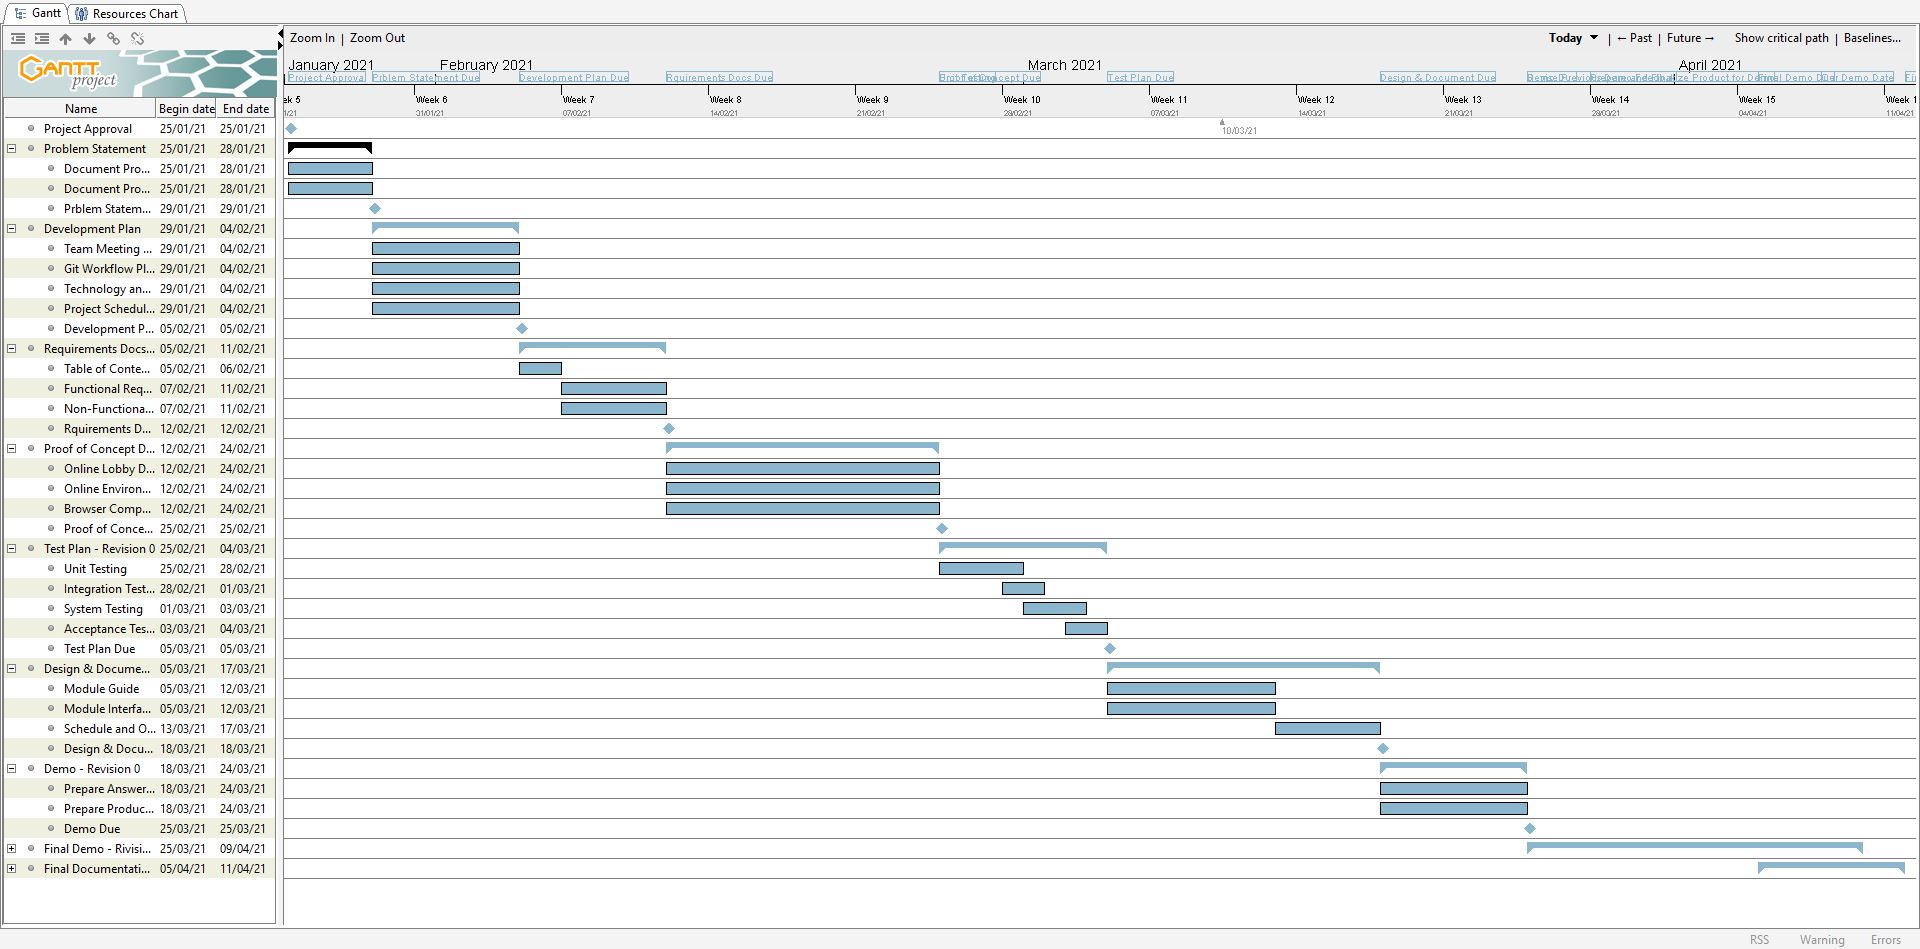
\includegraphics[width=16cm]{ProjectSchedule}
\caption{Project Schedule}
\label{fig:figure2}
\end{figure}


\subsection{Migration to the New Product}
N/A.

\subsection{Risks}

\subsubsection{Schedule Pressure}

This project contains many different time constraints, it will be the job of all team members to stay on top of the work but there is still a risk of falling behind schedule.

\subsubsection{Low Quality}

Many of the features in our project have never been attempted by any of the developers on the team, this may result in the project to be of lower quality than similar online games currently avaliable.

\subsection{Costs}

The majority of the software that will be used in the project will be free. The only costs that will be required is the cost of hosting a website on which the game will be played. These costs include \$17/year for the domain name and \$0.80/month to host the website on hostlinger.com.

\subsection{User Documentation and Training}

The game will have simplistic controls which can be seen on the Main Menu of the game, as well as a help button can be pressed in game to bring up the controls once the game has begun.

\subsection{Waiting Room}

Online leader-boards and accounts that can be logged into will not be released in this version of the project.

\subsection{Ideas for Solutions}
N/A

\bibliographystyle{plainnat}

\bibliography{SRS}

\newpage

\section{Appendix}

\subsection{Symbolic Parameters}

N/A


\end{document}